\chapter{Implementasi dan Pengujian}
\label{chap:Implementasi}

Pada bab ini akan ditunjukkan tampilan dari implementasi perangkat lunak dan juga bagaimana perangkat lunak diimplementasikan. Pengujian juga akan diterapkan pada perangkat lunak secara fungsional dan eksperimental. Hasil dari pegujian akan dijelaskan secara rinci dan sistemasi serta akan dibuat kesimpulan untuk pengujian yang telah dilakukan.


% \section{Implementasi Perangkat Lunak}
% \label{sec:implementasi-pl}

% \subsection{Instalasi}
% \label{sec:instalasi}

% \subsection{Antarmuka}
% \label{sec:antarmuka}

% \subsection{Randomisasi}
% \label{sec:randomisasi}


\section{Implementasi Antarmuka}
\label{sec:implementasi-antarmuka}

Antarmuka perangkat lunak diimplementasikan dengan memakai \textit{framework} antarmuka grafis berbasis bahasa pemograman Python yang bernama Kivy\footnote{https://kivy.org/\#home}. Implementasi antarmuka disesuaikan dengan rancangan antarmuka perangkat lunak yang telah dibuat pada bab~\ref{chap:perancangan}. Gambar~\ref{fig:antarmukautama} adalah tampilan antarmuka dari implementasi perangkat lunak.

\begin{figure}
	\centering
	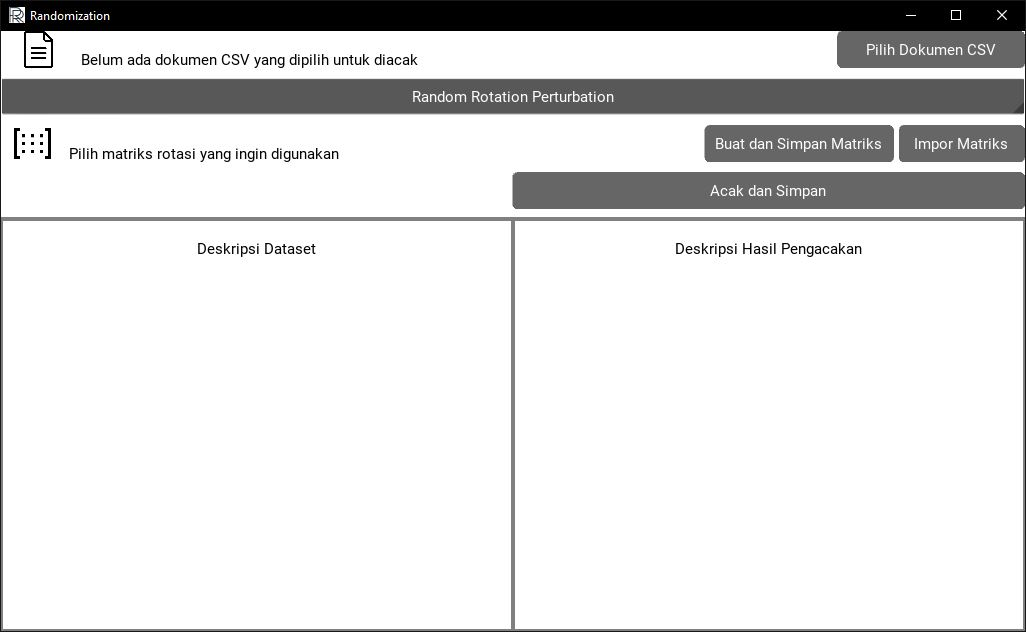
\includegraphics[scale=0.6]{antarmukautama}
	\caption{Tampilan perangkat lunak yang pertama ditampilkan saat perangkat lunak baru dibuka}
	\label{fig:antarmukautama}
\end{figure}

Antarmuka perangkat lunak mempunyai tiga buah bagian yang mempunyai fungsinya masing-masing. Ketiga bagian ini dapat dilihat pada Gambar~\ref{fig:antarmukautamabernomor} Pertama adalah bagian masukan dan pengaturan, terdapat pada bagian atas yang bernomor satu dan dikelilingi kotak merah. Kedua adalah bagian deskripsi dataset, terdapat pada bagian bawah sebelah kiri yang bernomor dua dan dikelilingi kotak biru. Terakhir adalah bagian deskripsi hasil randomisasi, terdapat pada bagian bawah sebelah kanan yang bernomor tiga dan dikelilingi kotak hijau. Ketiga bagian ini akan dijelaskan secara rinci pada subbab-subbab berikutnya.

\begin{figure}
	\centering
	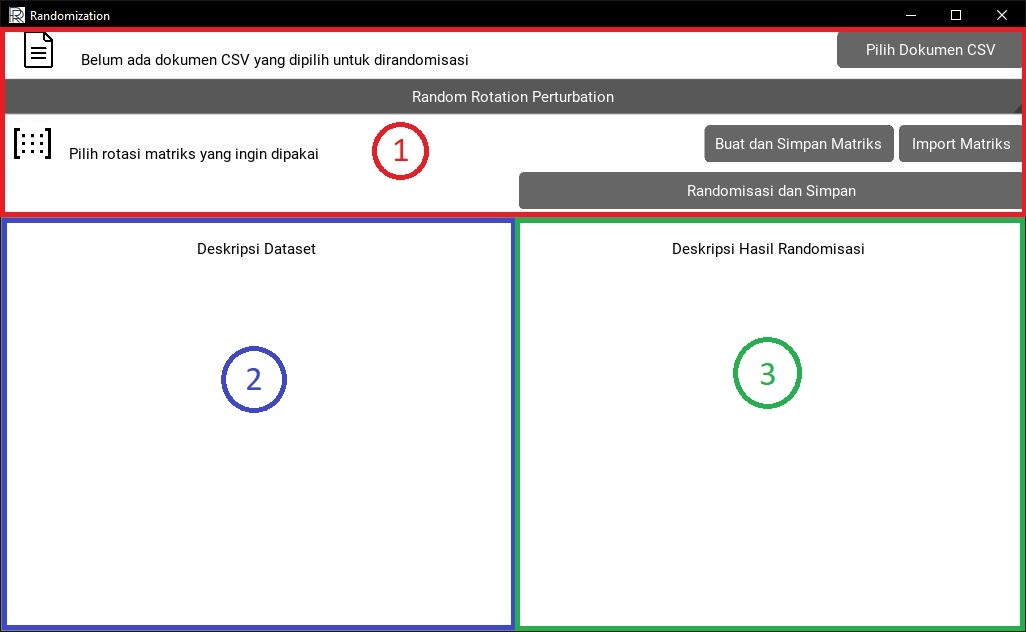
\includegraphics[scale=0.6]{antarmukautamabernomor}
	\caption{Bagian-bagian pada antarmuka perangkat lunak}
	\label{fig:antarmukautamabernomor}
\end{figure}

Perangkat lunak randomisasi ini mengimplementasikan dua buah teknik randomisasi yang berbeda yaitu \textit{Random Rotation Perturbation} dan \textit{Random Projection Perturbation}. Oleh karena itu, antarmuka perangkat lunak akan menyesuaikan dengan teknik yang dipilih oleh pengguna. Ketiga bagian antarmuka yang telah disebutkan tadi dengan otomatis akan berubah sesuai dengan teknik yang dipilih. Pada setiap subbab akan dijelaskan juga sekaligus perbedaan antarmuka teknik randomisasi satu dengan yang lainnya.

\subsection{Masukan dan Pengaturan}
\label{sec:masukanpengaturan}

Bagian masukan dan pengaturan menyediakan berbagai interaksi untuk pengguna dapat mengatur masukan yang perlu diberikan kepada perangkat lunak dan menerapkan teknik randomisasi yang diinginkan. Ada beberapa fungsi inti pada bagian ini yaitu masukan dataset berupa file \textit{comma-separated values} yang ingin dirandomisasi, memilih teknik randomisasi yang ingin digunakan, membuat baru dan memilih matriks rotasi atau proyeksi yang ingin digunakan, masukan nilai variabel Epsilon dan nilai variabel K untuk teknik \textit{Random Projection Perturbation}, dan sebuah tombol untuk menerapkan teknik randomisasi dan menyimpan hasilnya. Berikut akan dijelaskan secara rinci dengan gambar setiap fungsi tersebut yang dapat dilihat pada Gambar~\ref{fig:antarmukamasukanpengaturan} dan cara pemakaiannya yang benar secara berturut. 

\begin{figure}
	\centering
	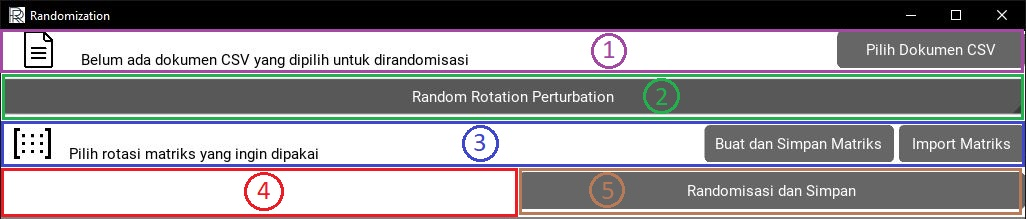
\includegraphics[scale=0.6]{antarmukamasukanpengaturan}
	\caption{Bagian antarmuka masukan dan pengaturan perangkat lunak}
	\label{fig:antarmukamasukanpengaturan}
\end{figure}

\subsubsection{Masukan Dataset}
\label{sec:masukandataset}

Pertama pengguna perlu memberikan masukan dataset yang ingin dirandomisasi berupa dokumen berjenis \textit{comma-separated values}. Perangkat lunak menyediakan fitur tersebut yang dapat dilihat pada Gambar~\ref{fig:antarmukamasukanpengaturan} yang terdapat pada bagian yang dikelilingi kotak berwarna merah dan bernomor satu. Pengguna dapat menekan tombol \textquotedblleft Pilih Dokumen CSV\textquotedblright~yang terletak pada ujung sebelah kanan. Tombol ini bertujuan untuk memilih dokumen yang ingin dirandomisasi pada direktori pengguna. Ketika tombol ditekan, perangkat lunak akan membuka jendela baru untuk memilih dokumen yang dapat dilihat pada gambar~\ref{fig:pilihdokumen}.

\begin{figure}
	\centering
	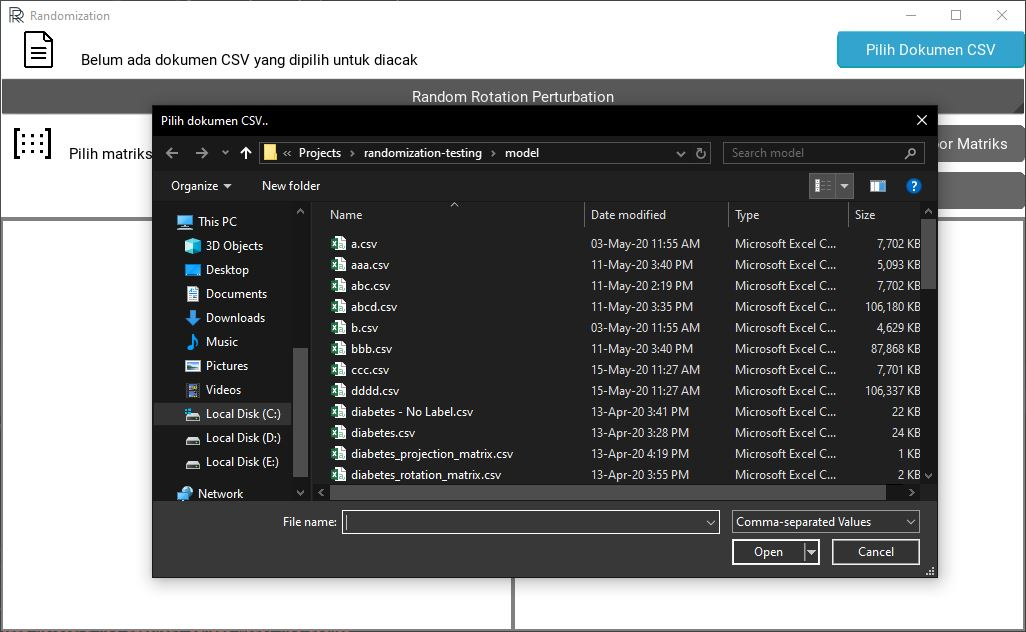
\includegraphics[scale=0.6]{pilihdokumen}
	\caption{Jendela untuk memilih dataset yang berupa dokumen CSV}
	\label{fig:pilihdokumen}
\end{figure}

Setelah pengguna memilih dataset yang diinginkan, perangkat lunak akan otomatis menuliskan lokasi dokumen yang dipilih berada. Perangkat lunak akan menampilkan lokasi dokumen tersebut pada bagian tengah sebelah kanan simbol dokumen dan sebelah kiri tombol \textquotedblleft Pilih Dokumen CSV\textquotedblright. Jika belum ada dataset yang dipilih maka perangkat lunak akan menampilkan label yang berupa kalimat \textquotedblleft Belum ada dokumen CSV yang dipilih untuk dirandomisasi\textquotedblright~yang menunjukkan bahwa belum ada dokumen yang dipilih oleh pengguna. Jika pengguna memilih ulang dokumen, maka secara otomatis juga perangkat lunak akan memperbaharui lokasi dokumen sesuai dokumen yang dipilih pengguna.

Apabila dokumen yang dipilih berukuran besar, maka perangkat lunak akan memakan sedikit waktu yang lebih lama. Dalam rangka memberitahukan kepada pengguna bahwa perangkat lunak sedang melakukan proses pemilihan dokumen, perangkat lunak akan menampilkan sebuah \textit{popup} yang memberitahukan bahwa proses pemilihan sedang berjalan dan perangkat lunak tidak berhenti bekerja maupun \textit{error} sehingga pengguna tidak bingung apabila perangkat lunak memakan waktu yang lebih lama untuk memproses dokumen yang dipilih. Tampilan antarmuka \textit{popup} tersebut dapat dilihat pada Gambar~\ref{fig:loadingmemilihdokumen}. Setelah dokumen dipilih pengguna dan perangkat lunak berhasil memproses dokumen tersebut, perangkat lunak akan memperbaharui lokasi dokumen dan menampilkan beberapa informasi dataset yang dipilih pada bagian deskripsi dataset yang akan dijelaskan pada subbab berikutnya. Tampilan antarmuka setelah pengguna memilih dokumen dapat dilihat pada Gambar~\ref{fig:dokumendipilih}

\begin{figure}
	\centering
	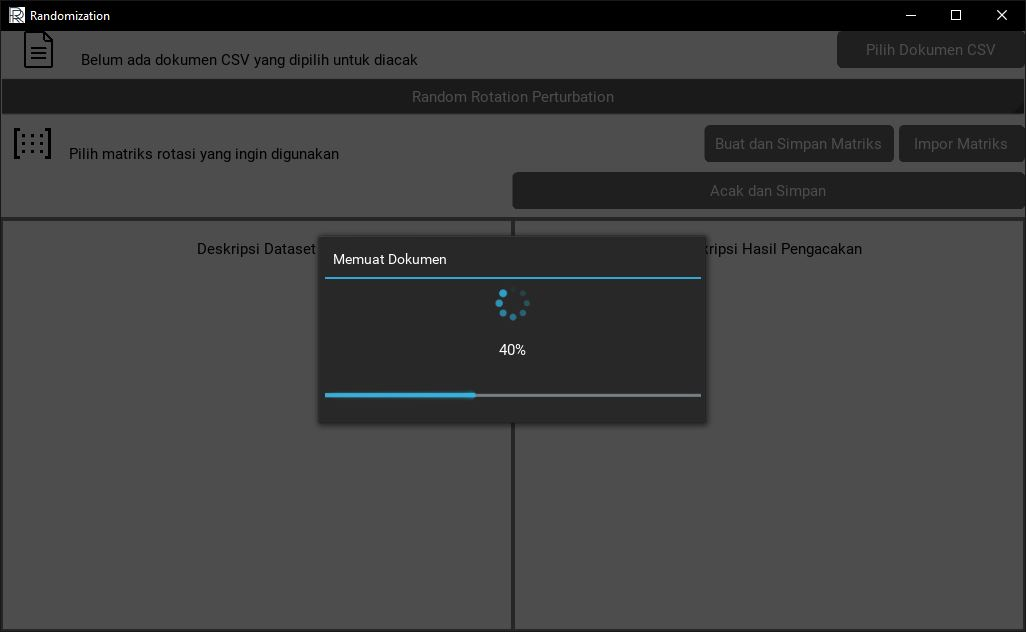
\includegraphics[scale=0.6]{loadingmemilihdokumen}
	\caption{Tampilan \textit{popup} yang ditampilkan saat proses berlangsung}
	\label{fig:loadingmemilihdokumen}
\end{figure}

\begin{figure}
	\centering
	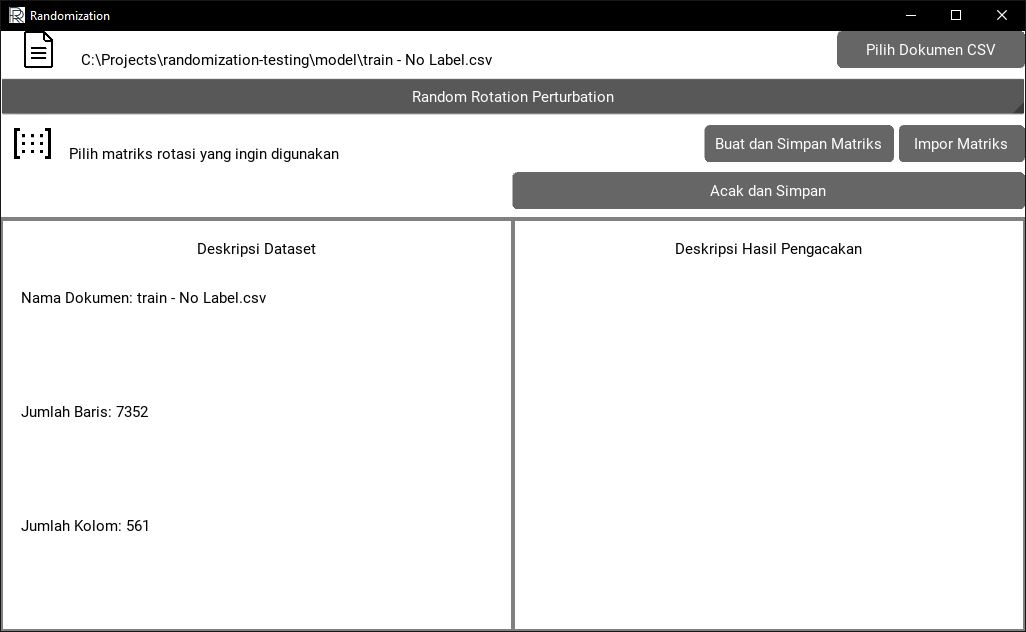
\includegraphics[scale=0.6]{dokumendipilih}
	\caption{Tampilan antarmuka setelah sebuah dokumen dipilih}
	\label{fig:dokumendipilih}
\end{figure}

Selain itu setelah pengguna memilih dokumen CSV, perangkat lunak akan membaca dokumen tersebut dan memproses isi dari dokumen tersebut menjadi dataset yang berupa matriks. Proses ini dilakukan sekali saja tepat setelah pengguna memilih dokumen dengan menekan tombol \textquotedblleft Pilih Dokumen CSV\textquotedblright. Oleh karena itu, apabila sebuah dokumen CSV diubah isinya setelah dokumen tersebut dipilih oleh pengguna maka perangkat lunak tetap akan menggunakan isi dari dokumen tersebut yang belum diubah. Pengguna harus berhati-hati apabila isi dokumen diubah maka pengguna juga harus memilih kembali dokumen yang sama tersebut walaupun perangkat lunak sudah menunjukkan lokasi dokumen yang digunakan adalah dokumen yang pengguna inginkan.

\subsubsection{Pemilihan Teknik Randomisasi}
\label{sec:pilihteknik}

Setelah pengguna memilih dataset yang ingin dirandomisasi, pengguna juga harus memilih teknik randomisasi apa yang ingin diterapkan terhadap dataset yang sudah dipilih. Pada awal perangkat lunak dibuka, secara otomatis teknik \textit{Random Rotation Perturbation} yang dipilih. Apabila pengguna ingin mengganti teknik yang ingin diterapkan pada dataset, pengguna dapat menekan tombol \textit{dropdown} yang bertuliskan nama teknik randomisasi. Tombol ini dapat dilihat pada Gambar~\ref{fig:antarmukamasukanpengaturan} yang dikelilingi kotak berwarna hijau dan bernomor dua.

Apabila pengguna menekan tombol ini maka perangkat lunak akan menampilkan \textit{dropdown} yang mempunyai dua buah opsi teknik randomisasi yaitu \textquotedblleft Random Rotation Perturbation\textquotedblright~dan \textquotedblleft Random Projection Perturbation\textquotedblright. Antarmuka tersebut dapat dilihat pada Gambar~\ref{fig:opsipilihteknik} yang dikelilingi oleh kotak merah. Pemilihan teknik ini juga akan memicu beberapa perubahan pada tampilan antarmuka perangkat lunak menyesuaikan dengan teknik yang dipilih. Beberapa perubahan pada perangkat lunak tersebut melingkupi bagian pembuatan dan pemilihan matriks, parameter teknik randomisasi, dan bagian randomisasi dan simpan yang akan dijelaskan setiap perubahan tersebut pada subbab berikutnya.

\begin{figure}
	\centering
	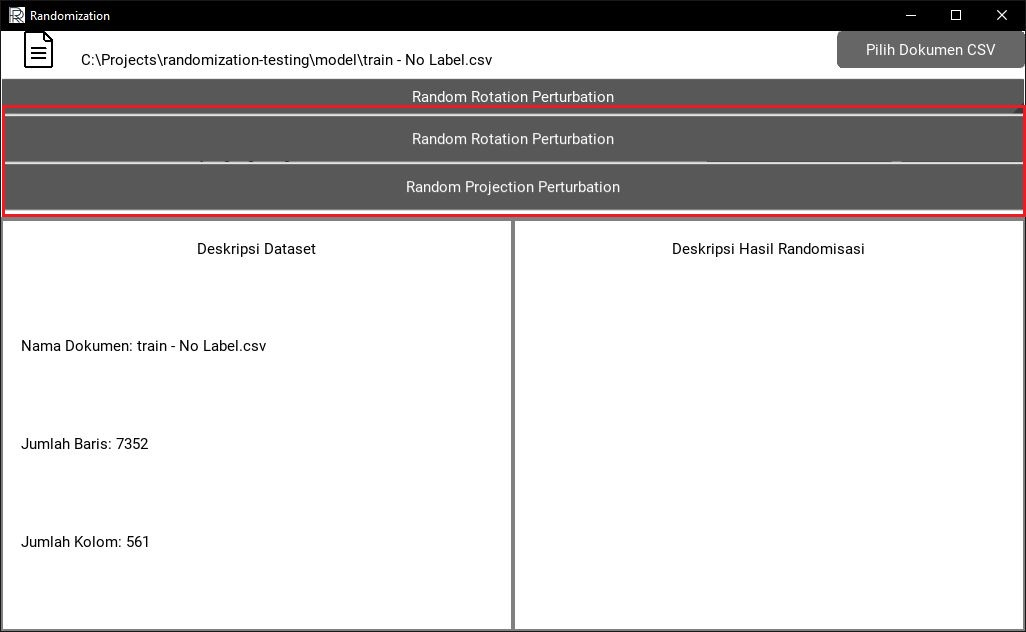
\includegraphics[scale=0.6]{opsipilihteknik}
	\caption{Tampilan antarmuka saat pengguna memilih teknik}
	\label{fig:opsipilihteknik}
\end{figure}

\subsubsection{Pembuatan dan Pemilihan Matriks}
\label{sec:pilihmatriks}

Setelah pengguna memilih teknik yang ingin diterapkan, pengguna harus memilih matriks yang diinginkan atau membuat baru. Matriks yang dimaksudkan adalah matriks rotasi atau matriks proyeksi sesuai teknik randomisasi yang dipilih. Apabila teknik \textit{Random Rotation Perturbation} yang dipilih maka perangkat lunak akan mengubah fungsi pembuatan dan pemilihan matriks ini menjadi matriks rotasi. Apabila teknik \textit{Random Projection Perturbation} yang dipilih maka perangkat lunak akan mengubah fungsi pembuatan dan pemilihan matriks ini menjadi matriks proyeksi. Perubahan ini dapat terlihat pada label yang berada di sebelah kanan simbol matriks apabila belum memilih atau membuat matriks maka label tersebut akan menampilkan kalimat \textquotedblleft Pilih matriks rotasi yang ingin digunakan\textquotedblright~atau \textquotedblleft Pilih matriks proyeksi yang ingin digunakan\textquotedblright. Bagian ini dapat dilihat pada Gambar~\ref{fig:antarmukamasukanpengaturan} yang dikelilingi oleh kotak berwarna hijau dan bernomor dua.

Ada dua buah tombol pada bagian ini yaitu \textquotedblleft Buat dan Simpan Matriks\textquotedblright~dan \textquotedblleft Import Matriks\textquotedblright. Tombol \textquotedblleft Buat dan Simpan Matriks\textquotedblright~mempunyai fungsi untuk membuat matriks rotasi atau proyeksi baru sesuai teknik randomisasi yang dipilih dan menyimpan matriks tersebut pada sebuah dokumen CSV baru yang dibuat oleh perangkat lunak pada direktori tertentu yang akan dipilih oleh pengguna. Pada saat perangkat lunak sedang memproses matriks tersebut, perangkat lunak akan menampilkan \textit{popup} memuat yang dapat dilihat pada Gambar~\ref{fig:buatsimpanmatriks}. \textit{Popup} ini juga akan tampil saat proses impor matriks dilakukan. Hasil matriks yang dibuat oleh perangkat lunak dapat digunakan kembali untuk lain kali sehingga rotasi atau proyeksi yang diterapkan akan sama dengan yang sebelumnya. 

Pengguna dapat melakukan impor matriks dengan cara menekan tombol \textquotedblleft Import Matriks\textquotedblright~untuk memilih matriks rotasi atau proyeksi yang diinginkan untuk diterapkan pada dataset. Matriks yang dipilih harus sesuai dengan dataset yang ingin dirandomisasi, misalnya apabila matriks rotasi yang dipilih memiliki dimensi yang berbeda dengan dataset maka perangkat lunak akan melarang impor matriks dilakukan karena randomisasi tidak dapat dilakukan. Perangkat lunak akan menampilkan \textit{popup} peringatan untuk pengguna yang dapat dilihat pada Gambar~\ref{fig:matrikstidaksesuai}. Apabila pengguna memilih teknik \textit{Random Projection Perturbation} dan pengguna mengimpor matriks proyeksi maka parameter variabel K akan terisi secara otomatis sesuai dengan matriks proyeksi yang diimpor.

\begin{figure}
	\centering
	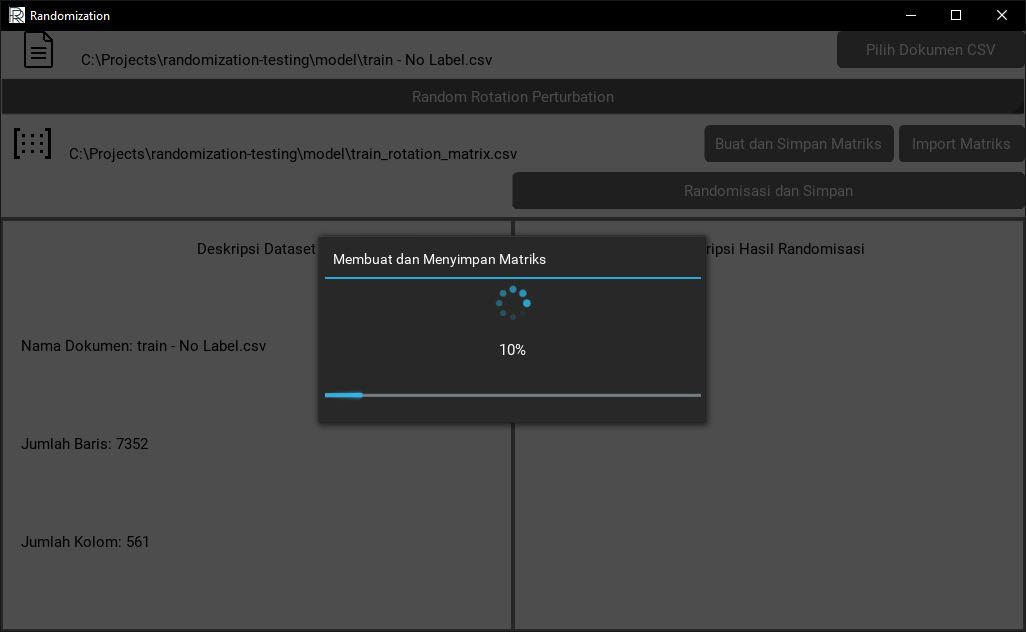
\includegraphics[scale=0.6]{buatsimpanmatriks}
	\caption{Tampilan antarmuka saat perangkat lunak membuat dan menyimpan matriks}
	\label{fig:buatsimpanmatriks}
\end{figure}

\begin{figure}
	\centering
	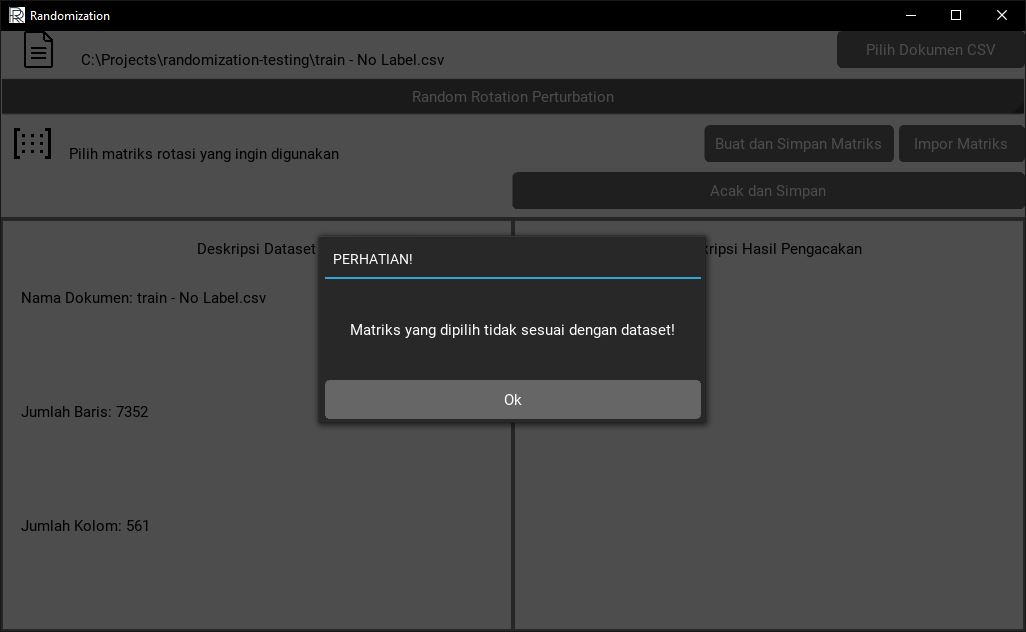
\includegraphics[scale=0.6]{matrikstidaksesuai}
	\caption{Tampilan \textit{popup} yang ditampilkan apabila matriks yang ingin diimpor tidak sesuai dengan dataset}
	\label{fig:matrikstidaksesuai}
\end{figure}

Apabila pengguna belum memilih dataset yang ingin dirandomisasi, pengguna tidak dapat membuat maupun impor matriks terlebih dahulu. Hal ini dikarenakan perlu ada proses pengecekan terlebih dahulu yang dilakukan perangkat lunak untuk memastikan dataset yang ingin dirandomisasi sudah sesuai persyaratan dan sesuai dengan matriks yang akan dipilih. Perangkat lunak akan melarang pengguna membuat maupun impor matriks dengan menampilkan sebuah \textit{popup} peringatan yang dapat dilihat pada Gambar~\ref{fig:larangmatriks}. Pada teknik \textit{Random Projection Perturbation}, pengguna baru bisa membuat matriks proyeksi apabila sudah memenuhi persyaratan yang diminta yaitu mengisi parameter teknik tersebut yang mana adalah variabel Epsilon dan variabel K.

\begin{figure}
	\centering
	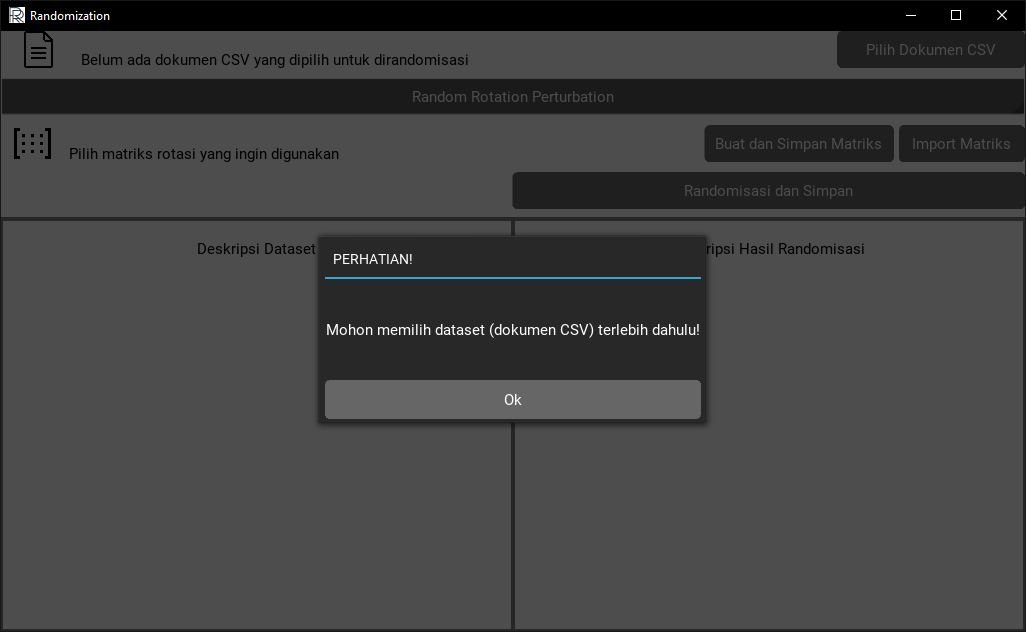
\includegraphics[scale=0.6]{larangmatriks}
	\caption{Tampilan \textit{popup} yang ditampilkan apabila pengguna belum memilih dataset yang ingin dirandomisasi}
	\label{fig:larangmatriks}
\end{figure}

\subsubsection{Parameter Teknik Randomisasi}
\label{sec:parameterteknik}

Perangkat lunak hanya meminta kepada pengguna parameter untuk teknik \textit{Random Projection Perturbation} saja apabila pengguna memilih teknik tersebut. Pada teknik \textit{Random Rotation Perturbation} tidak ada parameter yang perlu pengguna berikan. Ada dua buah parameter yang perlu pengguna berikan yaitu variabel Epsilon dan variabel K. Pengguna dapat memasukkan nilai kedua variabel tersebut dengan menekan kolom variabel tersebut masing-masing. Kedua buah parameter tersebut dapat dilihat antarmukanya pada Gambar~\ref{fig:parameterprojection}

\begin{figure}
	\centering
	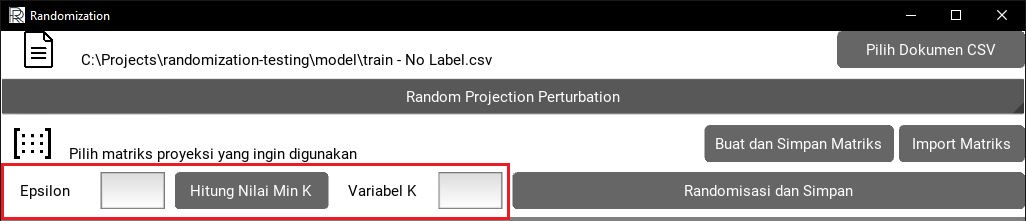
\includegraphics[scale=0.6]{parameterprojection}
	\caption{Tampilan antarmuka parameter teknik randomisasi \textit{Random Projection Perturbation}}
	\label{fig:parameterprojection}
\end{figure}

Seperti yang disinggung pada subbab sebelumnya antarmuka perangkat lunak akan menyesuaikan secara otomatis sesuai teknik yang dipilih pengguna. Pada bagian parameter teknik randomisasi, perangkat lunak akan menyembunyikan antarmuka parameter \textit{Random Projection Perturbation} apabila pengguna memilih teknik \textit{Random Rotation Perturbation}. Antarmuka tersebut dapat dilihat pada Gambar~\ref{fig:antarmukamasukanpengaturan} yang dikelilingi oleh kotak berwarna merah dan bernomor empat, dapat dilihat tidak ada parameter apapun yang tampil apabila teknik \textit{Random Rotation Perturbation} yang dipilih.

Selain dua buah parameter, pada bagian ini juga ada sebuah tombol yaitu \textquotedblleft Hitung Nilai Min K\textquotedblright~yang memiliki fungsi untuk menghitung nilai minimal variabel K yang pengguna berikan. Pada teknik \textit{Random Projection Perturbation}, ada beberapa persyaratan yang harus dipenuhi oleh pengguna dan salah satunya adalah variabel K yang diberikan harus melebihi sebuah nilai minimal yang dihitung berdasarkan ukuran dataset dan nilai variabel Epsilon. Oleh karena itu, sebelum tombol ini dapat berfungsi, pengguna harus memilih terlebih dahulu dataset yang ingin dirandomisasi dan memberikan masukan nilai variabel Epsilon yang sesuai dengan persyaratan variabel Epsilon yaitu nilainya lebih besar dari 0 dan kurang dari 1. Apabila pengguna belum memenuhi kedua persyaratan tersebut, tombol tidak akan berfungsi dan perangkat lunak akan menampilkan \textit{popup} peringatan yang dapat dilihat pada Gambar~\ref{fig:popuphitungk}. Nilai minimal variabel K akan ditampilkan pada bagian antarmuka deskripsi dataset yang akan dijelaskan pada subbab berikutnya.

\begin{figure}
	\centering
	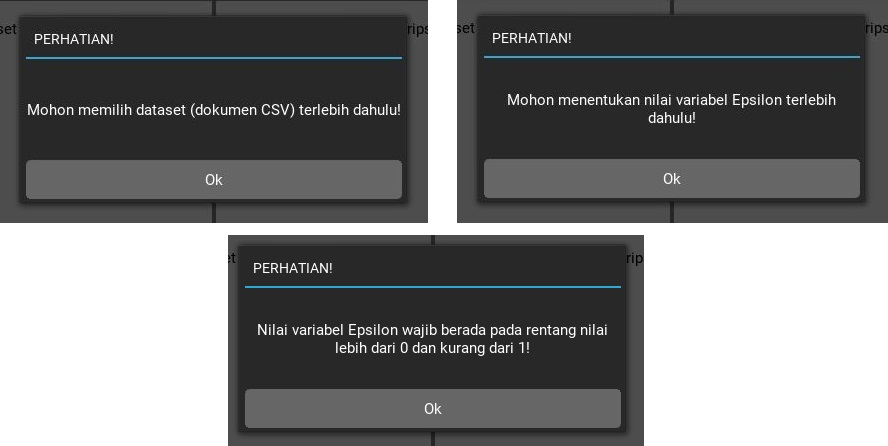
\includegraphics[scale=0.6]{popuphitungk}
	\caption{Tampilan \textit{popup} peringatan tombol \textquotedblleft Hitung Nilai Min K\textquotedblleft }
	\label{fig:popuphitungk}
\end{figure}

Perangkat lunak juga akan memberikan peringatan apabila nilai minimal K melebihi dimensi dari dataset yang ingin dirandomisasi karena salah satu persyaratan dari teknik \textit{Random Projection Perturbation} adalah nilai variabel K harus lebih kecil daripada jumlah dimensi pada dataset yang ingin dirandomisasi. Apabila pengguna melakukan impor matriks maka variabel K akan terisi secara otomatis dan pengguna harus menyesuaikan nilai variabel Epsilon dengan variabel K yang tidak boleh diubah oleh pengguna. 

\subsubsection{Randomisasi dan Simpan}
\label{sec:randomisasisimpan}

Setelah pengguna memberikan masukan yang sesuai dan mengatur pengaturan yang diinginkan maka pengguna telah dapat melakukan randomisasi dengan menekan tombol \textquotedblleft Randomisasi dan Simpan\textquotedblright. Tombol ini akan menerapkan teknik randomisasi yang dipilih oleh pengguna terhadap dataset yang ingin dirandomisasi menggunakan matriks yang telah dibuat atau dipilih oleh pengguna dan parameter-parameter yang pengguna berikan. Tampilan antarmuka saat proses randomisasi dilakukan perangkat lunak dapat dilihat pada Gambar~\ref{fig:loadingrandomisasi}.

\begin{figure}
	\centering
	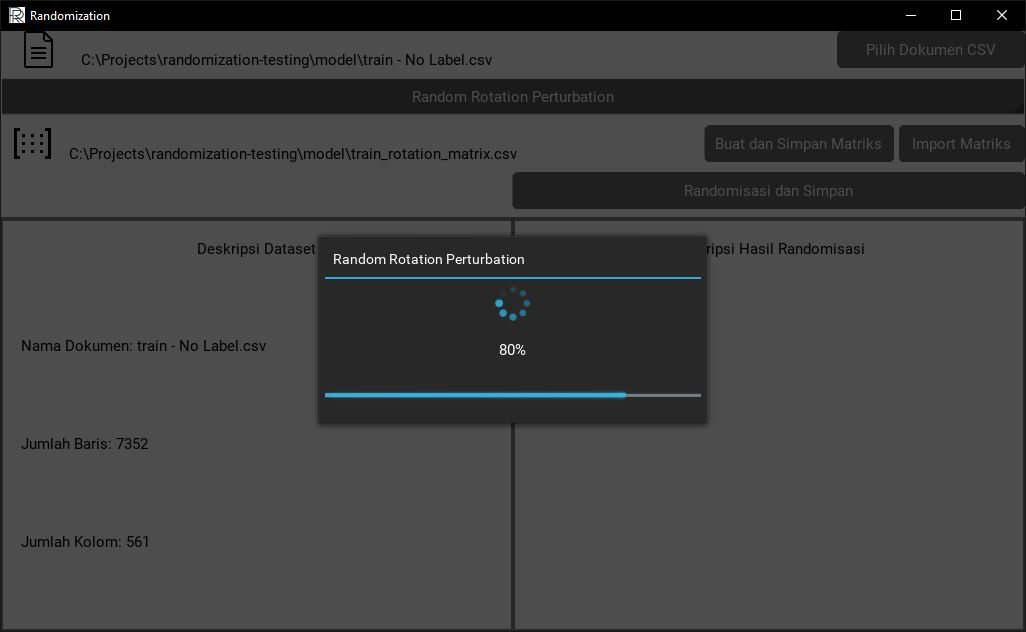
\includegraphics[scale=0.6]{loadingrandomisasi}
	\caption{Tampilan saat perangkat lunak sedang melakukan proses randomisasi}
	\label{fig:loadingrandomisasi}
\end{figure}

Setelah perangkat lunak berhasil melakukan randomisasi, perangkat lunak akan meminta pengguna untuk memilih direktori tempat penyimpanan dan nama dokumen hasil randomisasi. Perangkat lunak akan menyimpan hasil randomisasi dalam bentuk dokumen berjenis \textit{comma-separated values}. Jendela baru untuk memilih direktori penyimpanan akan ditampilkan perangkat lunak, apabila pengguna membatalkan atau dengan kata lain menutup jendela tersebut tanpa memilih direktori penyimpanan maka perangkat lunak tidak akan melanjutkan proses randomisasi dan dianggap gagal. Tampilan antarmuka \textit{popup} yang akan tampil setelah perangkat lunak berhasil melakukan proses randomisasi dan menyimpan hasilnya pada direktori yang pengguna pilih dapat dilihat pada Gambar~\ref{fig:popupberhasilrandomisasi}. Perangkat lunak juga akan menampilkan berbagai informasi hasil randomisasi pada bagian antarmuka deskripsi hasil randomisasi yang akan dijelaskan pada subbab berikutnya.

\begin{figure}
	\centering
	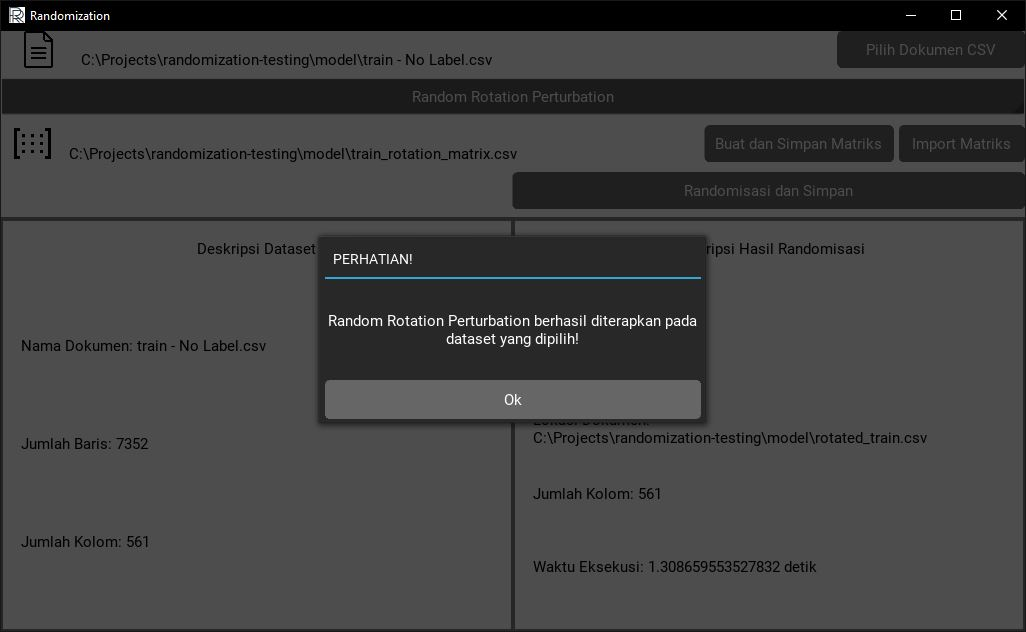
\includegraphics[scale=0.6]{popupberhasilrandomisasi}
	\caption{Tampilan \textit{popup} untuk memberitahukan pengguna bahwa randomisasi berhasil dilakukan}
	\label{fig:popupberhasilrandomisasi}
\end{figure}

Ada beberapa persyaratan yang harus dipenuhi oleh pengguna sebelum melakukan randomisasi yaitu memilih dataset yang ingin dirandomisasi, memilih teknik randomisasi yang diinginkan, membuat atau memilih matriks rotasi atau proyeksi, dan memberikan masukan nilai yang sesuai persyaratan yang ada kepada parameter-parameter teknik randomisasi. Apabila ada persyaratan yang tidak dipenuhi oleh pengguna maka perangkat lunak akan menampilkan \textit{popup} untuk memberikan peringatan kepada pengguna dan perangkat lunak tidak akan melanjutkan proses randomisasi. Perangkat lunak akan menampilkan \textit{popup} peringatan terhadap pelanggaran masing-masing persyaratan tersebut, salah satu contoh tampilan antarmuka \textit{popup} tersebut dapat dilihat pada Gambar~\ref{fig:popupdataset}.

\begin{figure}
	\centering
	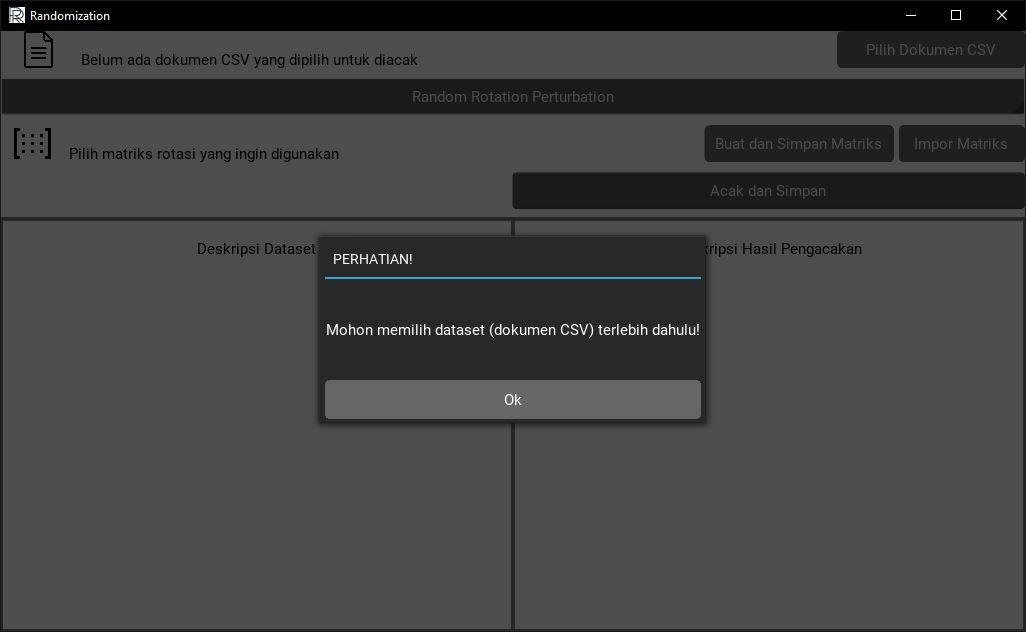
\includegraphics[scale=0.6]{popupdataset}
	\caption{Tampilan \textit{popup} peringatan apabila pengguna belum memilih dataset yang diinginkan untuk dirandomisasi}
	\label{fig:popupdataset}
\end{figure}

\subsection{Deskripsi Dataset}
\label{sec:deskripsidataset}

Pengguna dapat melihat berbagai informasi dokumen \textit{comma-separated values} yang dipilih sebagai dataset yang ingin dirandomisasi pada bagian antarmuka deskripsi dataset. Perangkat lunak akan menampilkan berbagai informasi dataset yaitu nama dokumen, jumlah baris dataset, jumlah kolom dataset, dan nilai minimal variabel K. Seperti yang disinggung pada subbab sebelumnya, pada awalnya nilai minimal variabel K belum diketahui karena belum dihitung. Pengguna harus mengisi variabel Epsilon dan menekan tombol \textquotedblleft Hitung Nilai Min K\textquotedblright~agar perangkat lunak menghitung nilai minimal variabel K dan dapat menampilkannya pada deskripsi dataset.

Bagian antarmuka deskripsi dataset ini akan selalu secara otomatis diperbaharui setiap pengguna memilih dataset baru. Tampilan antarmuka bagian deskripsi dataset dapat dilihat pada Gambar~\ref{fig:antarmukautamabernomor} yang dikelilingi oleh kotak berwarna biru dan bernomor dua. Apabila pengguna telah memilih dataset yang diinginkan untuk dirandomisasi maka perangkat lunak secara otomatis akan memperbaharui tampilan antarmuka deskripsi dataset yang dapat dilihat pada Gambar~\ref{fig:antarmukadeskripsidataset}

\begin{figure}
	\centering
	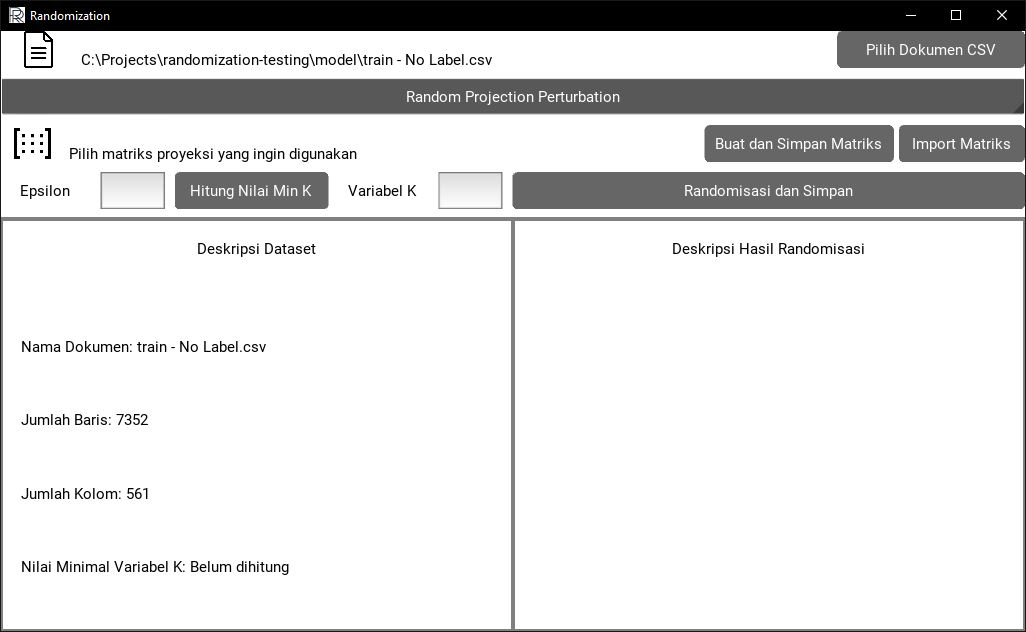
\includegraphics[scale=0.6]{antarmukadeskripsidataset}
	\caption{Tampilan antarmuka deskripsi dataset setelah pengguna memilih dataset yang ingin dirandomisasi}
	\label{fig:antarmukadeskripsidataset}
\end{figure}

\subsection{Deskripsi Hasil Randomisasi}
\label{sec:masukanpengaturan}

Perangkat lunak akan menampilkan isi dari deskripsi hasil randomisasi setelah pengguna menekan tombol \textquotedblleft Randomisasi dan Simpan\textquotedblright~dan perangkat lunak melakukan proses randomisasi. Bagian deskripsi hasil randomisasi ini akan menampilkan informasi-informasi yang berkaitan dengan hasil randomisasi dan deskripsi dataset yang baru. Informasi-informasi tersebut adalah status, lokasi dokumen, lokasi dokumen matriks yang dipakai, jumlah kolom, waktu eksekusi, nilai variabel Epsilon yang digunakan, dan nilai variabel K yang digunakan. Dua informasi terakhir tersebut hanya tampil apabila pengguna memilih teknik randomisasi \textquotedblleft Random Projection Perturbation\textquotedblright.

Bagian antarmuka deskripsi dataset ini akan selalu secara otomatis diperbaharui setiap pengguna memilih dataset baru. Tampilan antarmuka bagian deskripsi dataset dapat dilihat pada Gambar~\ref{fig:antarmukautamabernomor} yang dikelilingi oleh kotak berwarna biru dan bernomor dua. Apabila pengguna telah memilih dataset yang diinginkan untuk dirandomisasi maka perangkat lunak secara otomatis akan memperbaharui tampilan antarmuka deskripsi dataset yang dapat dilihat pada Gambar~\ref{fig:antarmukahasilrandomisasi}

\begin{figure}
	\centering
	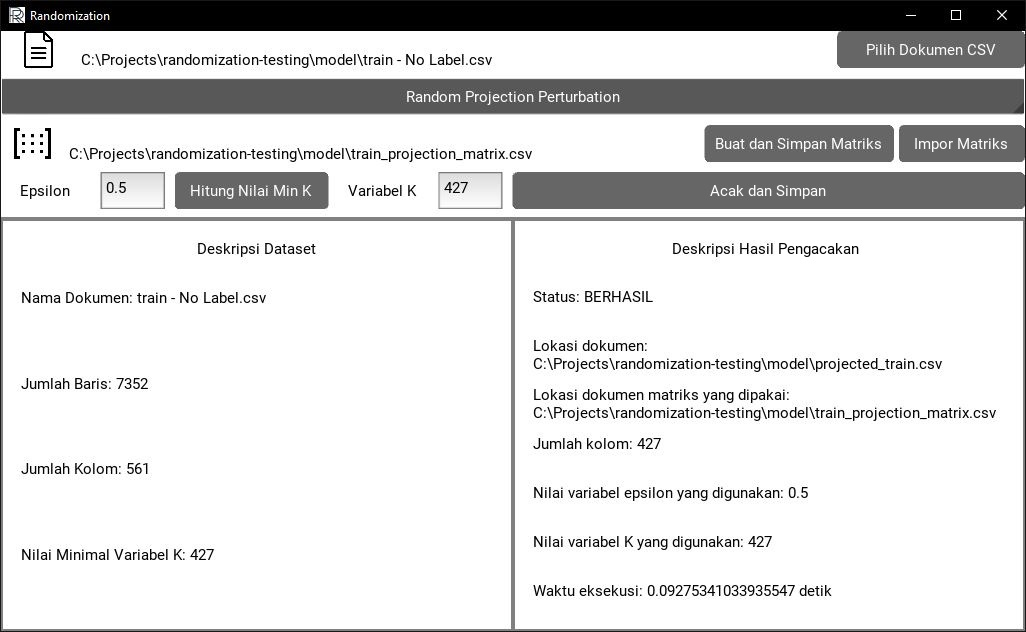
\includegraphics[scale=0.6]{antarmukahasilrandomisasi}
	\caption{Tampilan antarmuka deskripsi hasil randomisasi setelah perangkat berhasil melakukan randomisasi}
	\label{fig:antarmukahasilrandomisasi}
\end{figure}

\section{Pengujian Perangkat Lunak}
\label{sec:pengujianpl}

Pengujian perangkat lunak akan dibagi menjadi dua bagian yaitu pengujian fungsional dan pengujian eksperimental. Pengujian ini bertujuan untuk memastikan bahwa perangkat lunak randomisasi dapat bekerja dengan baik sebagaimana fungsinya dan menguji kualitas data yang dihasilkan perangkat lunak.

\subsection{Pengujian Fungsional}
\label{sec:pengujianfungsional}

Pengujian fungsional bertujuan untuk memastikan perangkat lunak randomisasi dapat menerapkan kedua teknik randomisasi yaitu \textit{Random Rotation Perturbation} dan \textit{Random Projection Perturbation} dengan baik terhadap dataset yang memenuhi syarat. Proses pengujian akan dilakukan dengan cara menerapkan kedua teknik tersebut dari awal memasukkan dataset sampai menghasilkan dataset yang telah dirandomisasi. Berikut pengujian pada setiap teknik randomisasi dengan menerapkan teknik penambangan data. Berikut pengujian pada setiap teknik randomisasi dengan menerapkan teknik penambangan data.

\subsubsection{Teknik \textit{Random Rotation Perturbation} dengan teknik penambangan data \textit{K-Nearest Neighbors}}
\label{sec:rrp-knn}

Pengujian teknik \textit{Random Rotation Perturbation} akan menggunakan dataset \textit{diabetes} yang berisi data kesehatan beberapa orang yang memiliki penyakit \textit{diabetes} dan tidak. Dataset ini memiliki 8 buah fitur dan sebuah label. Delapan buah fitur tersebut akan dirandomisasi dan diharapkan hasilnya akan mengacak dataset sehingga nilai tiap fitur tersebut berbeda dari aslinya. Selain itu, matriks rotasi harus dapat disimpan dan digunakan kembali untuk lain kali. Kemudian diterapkan teknik klasifikasi dengan algoritma \textit{K-nearest Neighbors} untuk menguji apakah dataset mempunyai akurasi model klasifikasi yang sama persis. Pengujian tersebut didasarkan pada sifat teknik \textit{Random Rotation Perturbation} yang menjamin jarak Euclidean setiap titik tidak berubah sama sekali.

Label pada dataset \textit{diabetes} yang ingin dirandomisasi harus dihilangkan terlebih dahulu agar hanya fitur dataset tersebut saja yang terandomisasi. Berikut akan ditampilkan 20 baris pertama dataset asli dan dataset yang telah dirandomisasi masing-masing pada Gambar~\ref{fig:diabetes_asli} dan Gambar~\ref{fig:rotated_diabetes}. Dapat dilihat pada gambar tersebut, dataset setelah dirandomisasi memiliki nilai yang sangat berbeda dengan aslinya, bahkan nilai yang sama pada beberapa baris di dataset asli tidak sama dengan dataset yang telah dirandomisasi pada baris yang sama seperti pada kolom \textit{insulin} baris satu sampai tiga memiliki nilai 0 pada dataset asli tetap pada dataset yang telah dirandomisasi ketiga baris tersebut memiliki nilai yang berbeda antara satu dengan yang lainnya.

\begin{figure}
	\centering
	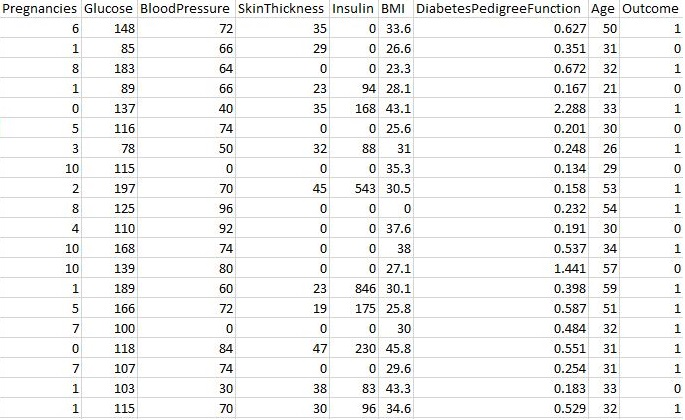
\includegraphics[scale=0.9]{diabetes_asli}
	\caption{Dua puluh baris pertama dataset \textit{diabetes} asli}
	\label{fig:diabetes_asli}
\end{figure}

\begin{figure}
	\centering
	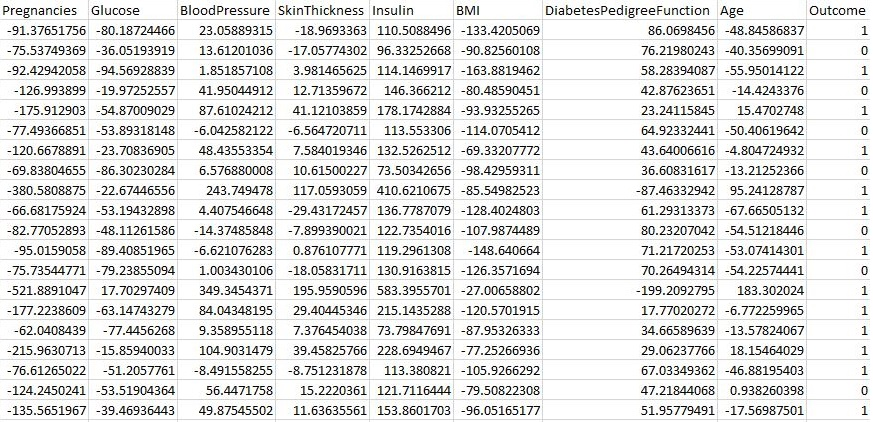
\includegraphics[scale=0.71]{rotated_diabetes}
	\caption{Dua puluh baris pertama dataset \textit{diabetes} setelah dirandomisasi}
	\label{fig:rotated_diabetes}
\end{figure}

Teknik penambangan data \textit{K-nearest Neighbors} diterapkan menggunakan delapan buah fitur yang ada. Dataset akan dibagi dua menjadi \textit{train set} dan \textit{test set} yang masing-masing berguna untuk melatih model dan menguji akurasi model. Akurasi akan dihitung dengan jumlah tetangga (nilai \textit{k}) dari 1 sampai 20. Nilai akurasi pada dataset asli dan dataset yang telah dirandomisasi masing-masing dapat dilihat pada Listing~\ref{diabetes_akurasi_asli} dan Listing~\ref{diabetes_akurasi_randomisasi}. Implementasi kode teknik penambangan data ini diterapkan dengan bahasa pemograman Python dan dibantu oleh \textit{library} Scikit-learn. 

\noindent\begin{minipage}{.48\textwidth}
\begin{lstlisting}[caption=Akurasi Dataset Asli,frame=tlrb, label=diabetes_akurasi_asli]{Name}
Akurasi setiap K pada training set 
dataset asli: 
1: 1.0
2: 0.8543478260869565
3: 0.8456521739130435
4: 0.808695652173913
5: 0.7891304347826087
6: 0.7847826086956522
7: 0.7869565217391304
8: 0.7782608695652173
9: 0.7869565217391304
10: 0.7673913043478261
11: 0.7804347826086957
12: 0.7673913043478261
13: 0.7760869565217391
14: 0.7760869565217391
15: 0.7673913043478261
16: 0.7608695652173914
17: 0.7673913043478261
18: 0.7739130434782608
19: 0.7760869565217391
20: 0.7717391304347826

Akurasi setiap K pada test set 
dataset asli: 
1: 0.6785714285714286
2: 0.6948051948051948
3: 0.685064935064935
4: 0.7077922077922078
5: 0.7012987012987013
6: 0.724025974025974
7: 0.7305194805194806
8: 0.7012987012987013
9: 0.7142857142857143
10: 0.7207792207792207
11: 0.7142857142857143
12: 0.7077922077922078
13: 0.7077922077922078
14: 0.7305194805194806
15: 0.7305194805194806
16: 0.7337662337662337
17: 0.7207792207792207
18: 0.7337662337662337
19: 0.724025974025974
20: 0.7337662337662337
\end{lstlisting}
\end{minipage}\hfill
\begin{minipage}{.48\textwidth}
\begin{lstlisting}[caption=Akurasi Dataset Randomisasi,frame=tlrb, label=diabetes_akurasi_randomisasi]{Name}
Akurasi setiap K pada training set 
dataset randomisasi: 
1: 1.0
2: 0.8543478260869565
3: 0.8456521739130435
4: 0.808695652173913
5: 0.7891304347826087
6: 0.7847826086956522
7: 0.7869565217391304
8: 0.7782608695652173
9: 0.7869565217391304
10: 0.7673913043478261
11: 0.7804347826086957
12: 0.7673913043478261
13: 0.7760869565217391
14: 0.7760869565217391
15: 0.7673913043478261
16: 0.7608695652173914
17: 0.7673913043478261
18: 0.7739130434782608
19: 0.7760869565217391
20: 0.7717391304347826

Akurasi setiap K pada test set 
dataset randomisasi: 
1: 0.6785714285714286
2: 0.6948051948051948
3: 0.685064935064935
4: 0.7077922077922078
5: 0.7012987012987013
6: 0.724025974025974
7: 0.7305194805194806
8: 0.7012987012987013
9: 0.7142857142857143
10: 0.7207792207792207
11: 0.7142857142857143
12: 0.7077922077922078
13: 0.7077922077922078
14: 0.7305194805194806
15: 0.7305194805194806
16: 0.7337662337662337
17: 0.7207792207792207
18: 0.7337662337662337
19: 0.724025974025974
20: 0.7337662337662337
\end{lstlisting}
\end{minipage}

Dapat dilihat pada kedua listing tersebut akurasi \textit{training set} dan \textit{test set} pada kedua dataset sama persis. Hal ini dikarenakan jarak Euclidean kedua buah dataset tidak berubah sama sekali. Oleh karena itu, perangkat lunak berhasil menerapkan dengan baik teknik \textit{Random Rotation Perturbation} untuk teknik penambangan data klasifikasi.

\subsubsection{Teknik \textit{Random Rotation Perturbation} dengan teknik penambangan data \textit{K-means}}
\label{sec:rrp-kmeans}

Pengujian teknik \textit{Random Rotation Perturbation} akan menggunakan dataset \textit{mall\_customers} yang berisi informasi pribadi pelanggan sebuah mall. Dataset ini memiliki empat buah fitur yaitu jenis kelamin, umur, penghasilan, dan skor pengeluaran. empat buah fitur tersebut akan dirandomisasi dan diharapkan hasilnya akan mengacak dataset sehingga nilai tiap fitur tersebut berbeda dari aslinya. Selain itu, matriks rotasi harus dapat disimpan dan digunakan kembali untuk lain kali. Kemudian diterapkan teknik \textit{clustering} dengan algoritma \textit{K-means} untuk menguji apakah dataset menghasilkan kluster dan bentuk yang sama dengan sudut yang berbeda saat divisualisasikan. Pengujian tersebut didasarkan pada sifat teknik \textit{Random Rotation Perturbation} yang menjamin jarak Euclidean setiap titik tidak berubah sama sekali.

Berikut akan ditampilkan 20 baris pertama dataset asli dan dataset yang telah dirandomisasi masing-masing pada Gambar~\ref{fig:mall_customers_asli} dan Gambar~\ref{fig:rotated_mall_customers}. Dapat dilihat pada gambar tersebut, dataset setelah dirandomisasi memiliki nilai yang sangat berbeda dengan aslinya.

\begin{figure}
	\centering
	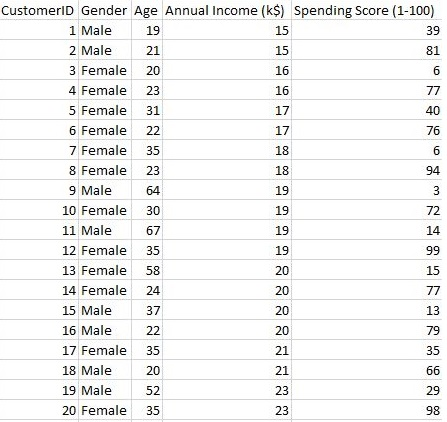
\includegraphics[scale=0.9]{mall_customers_asli}
	\caption{Dua puluh baris pertama dataset \textit{mall\_customers} asli}
	\label{fig:mall_customers_asli}
\end{figure}

\begin{figure}
	\centering
	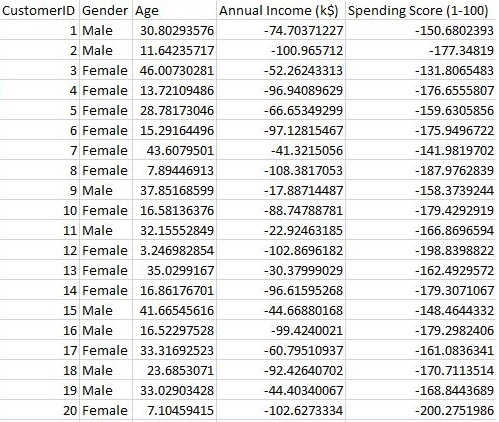
\includegraphics[scale=0.71]{rotated_mall_customers}
	\caption{Dua puluh baris pertama dataset \textit{mall\_customers} setelah dirandomisasi}
	\label{fig:rotated_mall_customers}
\end{figure}

Teknik penambangan data \textit{K-means} diterapkan menggunakan empat buah fitur yang ada. Akurasi akan dihitung dengan jumlah tetangga (nilai \textit{k}) dari 1 sampai 20. Visualisasi \textit{cluster} pada dataset asli dan dataset yang telah dirandomisasi masing-masing dapat dilihat pada Gambar~\ref{fig:kmeans_mall_asli} dan Gambar~\ref{fig:kmeans_mall_rotated}. Implementasi kode teknik penambangan data ini diterapkan dengan bahasa pemograman Python dan dibantu oleh \textit{library} Scikit-learn. 

\begin{figure}
	\centering
	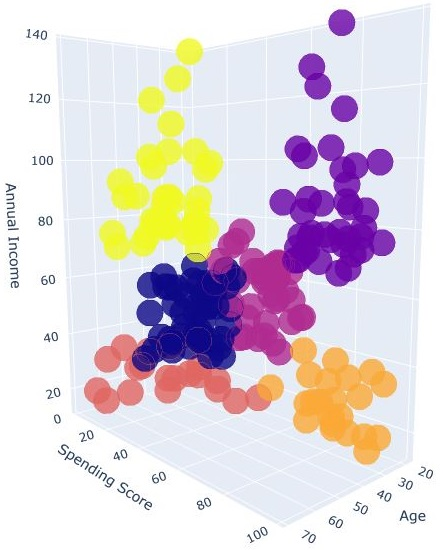
\includegraphics[scale=1]{kmeans_mall_asli}
	\caption{Visualisasi \textit{cluster} pada dataset yang asli}
	\label{fig:kmeans_mall_asli}
\end{figure}

\begin{figure}
	\centering
	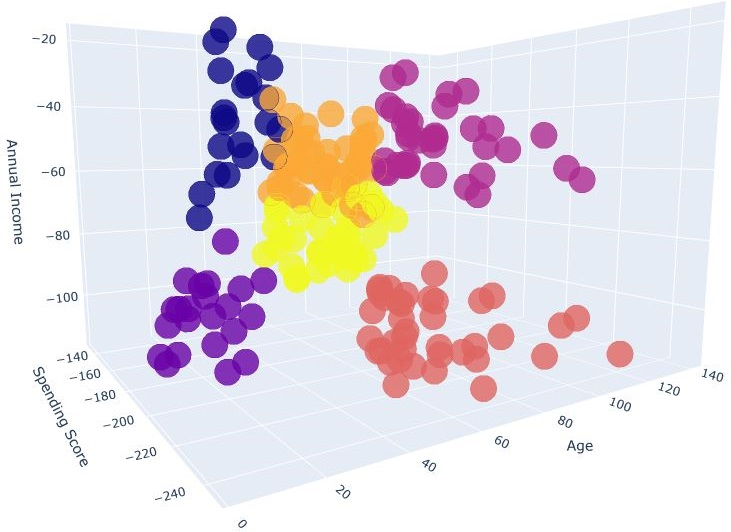
\includegraphics[scale=0.7]{kmeans_mall_rotated}
	\caption{Visualisasi \textit{cluster} pada dataset yang telah dirotasi}
	\label{fig:kmeans_mall_rotated}
\end{figure}

Dapat dilihat pada kedua \textit{scatter plot} tersebut \textit{cluster} yang dihasilkan sama yaitu 6 \textit{cluster} dan bentuk dari \textit{cluster-cluster} tersebut sama walaupun titik-titik yang ada memiliki lokasi yang berbeda. \textit{Adjusted Rand Index} pada kedua model tersebut memiliki nilai 1 yang berarti anggota \textit{cluster} pada setiap cluster antara kedua model tersebut sama persis. Hal ini dikarenakan jarak Euclidean kedua buah dataset tidak berubah sama sekali. Oleh karena itu, perangkat lunak berhasil menerapkan dengan baik teknik \textit{Random Rotation Perturbation} untuk penambangan data \textit{clustering}.

\subsubsection{Teknik \textit{Random Projection Perturbation} dengan teknik penambangan data \textit{K-Nearest Neighbors}}
\label{sec:rpp-knn}

Pengujian teknik \textit{Random Projection Perturbation} akan menggunakan dataset \textit{mobile\_sensor} yang berisi data sensor \textit{smartphone} banyak orang yang sedang melakukan aktivitas tertentu seperti berdiri, duduk, berjalan, berjalan menanjak, berjalan menurun, dan lain-lain. Dataset ini memiliki 561 buah fitur dan sebuah label. Seluruh fitur tersebut akan dirandomisasi dan diharapkan hasilnya akan mengacak dataset sehingga nilai tiap fitur tersebut berbeda dari aslinya. Selain itu, matriks proyeksi harus dapat disimpan dan digunakan kembali untuk lain kali. Kemudian diterapkan teknik klasifikasi dengan algoritma \textit{K-nearest Neighbors} untuk menguji apakah dataset mempunyai akurasi model klasifikasi yang hampir sama. Pengujian tersebut didasarkan pada sifat teknik \textit{Random Projection Perturbation} yang menjamin jarak Euclidean setiap titik tidak berubah jauh dengan besar \textit{error} yang ditentukan pengguna.

Label pada dataset \textit{mobile\_sensor} yang ingin dirandomisasi harus dihilangkan terlebih dahulu agar hanya fitur dataset tersebut saja yang terandomisasi. Berikut akan ditampilkan 7 fitur terakhir serta label pada 20 baris pertama dataset asli dan dataset yang telah dirandomisasi masing-masing pada Gambar~\ref{fig:mobile_sensor_asli} dan Gambar~\ref{fig:projected_mobile_sensor}. Dapat dilihat pada gambar tersebut, dataset setelah dirandomisasi memiliki nilai yang sangat berbeda dengan aslinya. 

\begin{figure}
	\centering
	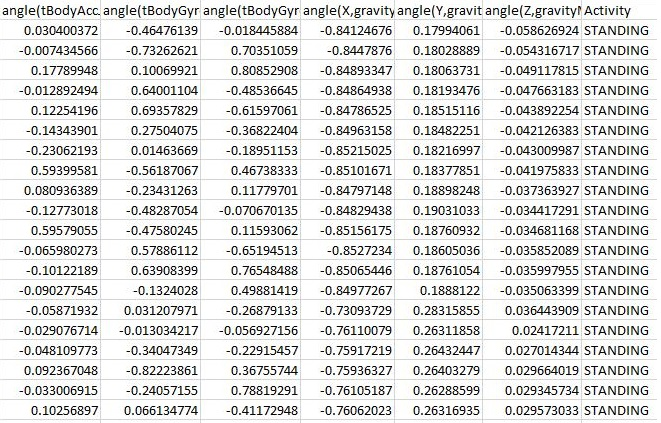
\includegraphics[scale=0.9]{mobile_sensor_asli}
	\caption{Dua puluh baris pertama dataset \textit{mobile\_sensor} yang asli}
	\label{fig:mobile_sensor_asli}
\end{figure}

\begin{figure}
	\centering
	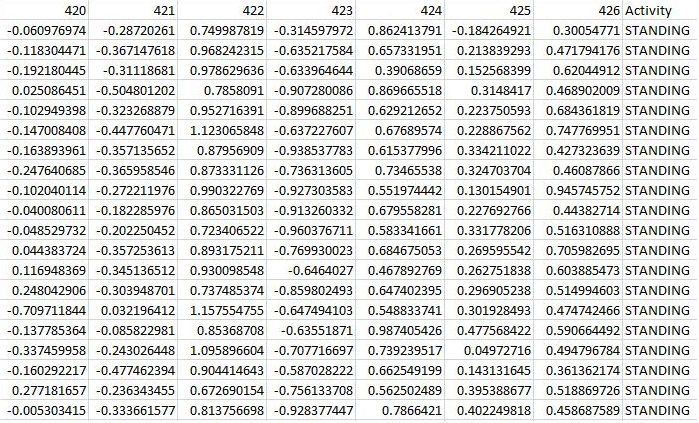
\includegraphics[scale=0.8]{projected_mobile_sensor}
	\caption{Dua puluh baris pertama dataset \textit{mobile\_sensor} setelah dirandomisasi}
	\label{fig:projected_mobile_sensor}
\end{figure}

Teknik penambangan data \textit{K-nearest Neighbors} diterapkan menggunakan delapan buah fitur yang ada. Dataset akan dibagi dua menjadi \textit{train set} dan \textit{test set} yang masing-masing berguna untuk melatih model dan menguji akurasi model. Akurasi akan dihitung dengan jumlah tetangga (nilai \textit{k}) dari 1 sampai 20. Nilai akurasi pada dataset asli dan dataset yang telah dirandomisasi masing-masing dapat dilihat pada Listing~\ref{mobile_sensor_akurasi_asli} dan Listing~\ref{mobile_sensor_akurasi_randomisasi}. Implementasi kode teknik penambangan data ini diterapkan dengan bahasa pemograman Python dan dibantu oleh \textit{library} Scikit-learn. 

\noindent\begin{minipage}{.48\textwidth}
\begin{lstlisting}[caption=Akurasi Dataset Asli,frame=tlrb, label=mobile_sensor_akurasi_asli]{Name}
Akurasi setiap K pada 
training set dataset asli: 
1: 1.0
2: 0.9887105549510338
3: 0.9919749727965179
4: 0.9862622415669206
5: 0.984221980413493
6: 0.984221980413493
7: 0.9817736670293797
8: 0.9790533188248096
9: 0.9771490750816104
10: 0.9764689880304679
11: 0.9741566920565833
12: 0.9734766050054406
13: 0.9721164309031556
14: 0.9713003264417845
15: 0.9691240478781284
16: 0.9685799782372143
17: 0.9674918389553863
18: 0.9681719260065288
19: 0.9659956474428727
20: 0.9665397170837867

Akurasi setiap K pada 
test set dataset asli: 
1: 0.8785205293518833
2: 0.8659653885307091
3: 0.8907363420427553
4: 0.8934509670851714
5: 0.9002375296912114
6: 0.9019341703427214
7: 0.9022734984730234
8: 0.9060061079063454
9: 0.9053274516457415
10: 0.9066847641669494
11: 0.9039701391245334
12: 0.9029521547336274
13: 0.9056667797760435
14: 0.9049881235154394
15: 0.9046487953851374
16: 0.9077027485578555
17: 0.9070240922972514
18: 0.9077027485578555
19: 0.9070240922972514
20: 0.9056667797760435
\end{lstlisting}
\end{minipage}\hfill
\begin{minipage}{.48\textwidth}
\begin{lstlisting}[caption=Akurasi Dataset Randomisasi,frame=tlrb, label=mobile_sensor_akurasi_randomisasi]{Name}
Akurasi setiap K pada training set 
dataset randomisasi: 
1: 1.0
2: 0.984221980413493
3: 0.9896626768226333
4: 0.9835418933623504
5: 0.9828618063112078
6: 0.9797334058759521
7: 0.9782372143634385
8: 0.9759249183895539
9: 0.9736126224156693
10: 0.9737486398258978
11: 0.9721164309031556
12: 0.9717083786724701
13: 0.9691240478781284
14: 0.9683079434167573
15: 0.9666757344940152
16: 0.9658596300326442
17: 0.9640914036996736
18: 0.9640914036996736
19: 0.9623231773667029
20: 0.9623231773667029

Akurasi setiap K pada test set 
dataset randomisasi: 
1: 0.8649474041398032
2: 0.8578215134034611
3: 0.8775025449609772
4: 0.8781812012215813
5: 0.8812351543942993
6: 0.8870037326094333
7: 0.8903970139124533
8: 0.8897183576518494
9: 0.8917543264336614
10: 0.8941296233457754
11: 0.8907363420427553
12: 0.8914149983033594
13: 0.8934509670851714
14: 0.8951476077366813
15: 0.8954869358669834
16: 0.8954869358669834
17: 0.8982015609093994
18: 0.8975229046487954
19: 0.8992195453003053
20: 0.9002375296912114
\end{lstlisting}
\end{minipage}

Dapat dilihat pada kedua listing tersebut akurasi \textit{test set} pada kedua dataset berbeda. Akurasi \textit{test set} tertinggi pada dataset asli adalah sebesar 0.9077027485578555 dengan nilai \textit{k} sebesar 16. Sementara pada dataset yang telah dirandomisasi, akurasi \textit{test set} tertingginya adalah sebesar 0.9002375296912114 dengan nilai \textit{k} sebesar 20. Jika dihitung perbedaan akurasinya adalah sebesar 0.0074652188666441 yang mana relatif kecil tetapi ada perbedaan pada nilai \textit{k} yang memiliki akurasi tertinggi. Perbedaan nilai \textit{k} ini akan diuji lebih lanjut pada pengujian eksperimental. Dengan perbedaan akurasi yang relatif kecil dan dataset yang telah dirandomisasi teracak dengan baik maka dapat disimpulkan perangkat lunak berhasil menerapkan teknik \textit{Random Projection Perturbation} untuk teknik penambangan data \textit{clustering}.

\subsubsection{Teknik \textit{Random Projection Perturbation} dengan teknik penambangan data \textit{K-means}}
\label{sec:rpp-kmeans}

Pengujian teknik \textit{Random Projection Perturbation} akan menggunakan dataset \textit{mobile\_sensor} yang sama seperti sebelumnya dan dapat dilihat pada Gambar~\ref{fig:mobile_sensor_asli} dan Gambar~\ref{fig:projected_mobile_sensor}. Dataset ini akan diterapkan teknik \textit{clustering} dengan algoritma \textit{K-means} untuk menguji apakah dataset menghasilkan kluster dan bentuk yang sama dengan sudut yang berbeda saat divisualisasikan. Pengujian tersebut didasarkan pada sifat teknik \textit{Random Projection Perturbation} yang menjamin jarak Euclidean setiap titik tidak berubah jauh dengan besar \textit{error} yang ditentukan pengguna.

Sebelum melakukan teknik \textit{clustering} dengan algoritma \textit{K-means}, dataset yang memiliki fitur yang sangat banyak tersebut dimensinya harus direduksi terlebih dahulu agar model dapat divisualisasikan dengan mudah. Dataset yang akan di\textit{cluster} akan direduksi dimensinya sampai hanya memiliki 2 dimensi. Reduksi dimensi dilakukan dengan menerapkan teknik \textit{Principal Component Analysis} yang sudah umum digunakan saat penambangan data dan hasilnya relatif baik.

Teknik penambangan data \textit{K-means} diterapkan menggunakan dua buah fitur yang ada hasil dari teknik \textit{Principal Component Analysis}. Model \textit{K-means} akan dibuat dengan nilai \textit{k} yang terbaik dihitung menggunakan metode Elbow dan nilai \textit{k} yang memiliki \textit{Sillhoutte Score} tertinggi. Visualisasi \textit{cluster} pada dataset asli dan dataset yang telah dirandomisasi masing-masing dapat dilihat pada Gambar~\ref{fig:kmeans_mobile_sensor_asli} dan Gambar~\ref{fig:kmeans_mobile_sensor_randomisasi}. Implementasi kode teknik penambangan data ini diterapkan dengan bahasa pemograman Python dan dibantu oleh \textit{library} Scikit-learn. 

\begin{figure}
	\centering
	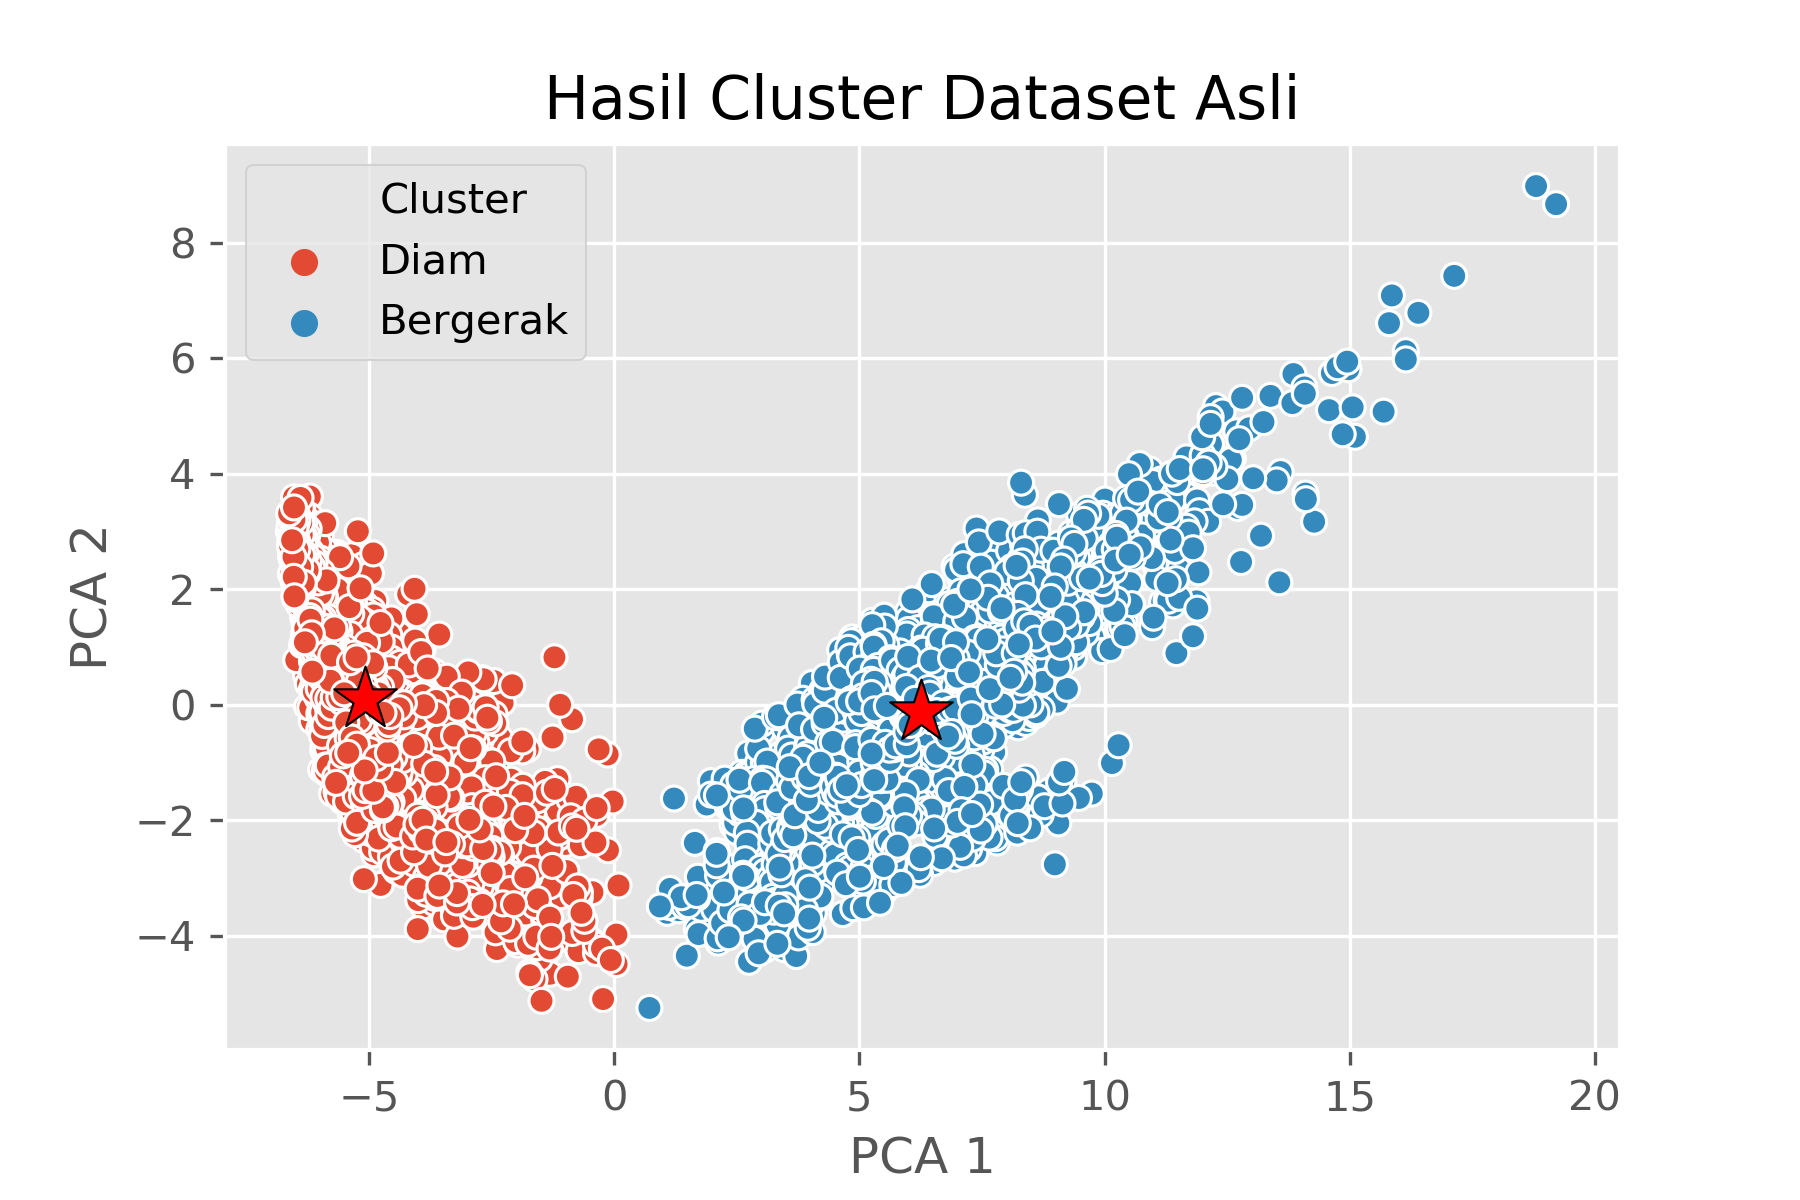
\includegraphics[scale=1]{kmeans_mobile_sensor_asli}
	\caption{Visualisasi \textit{cluster} pada dataset yang asli}
	\label{fig:kmeans_mobile_sensor_asli}
\end{figure}

\begin{figure}
	\centering
	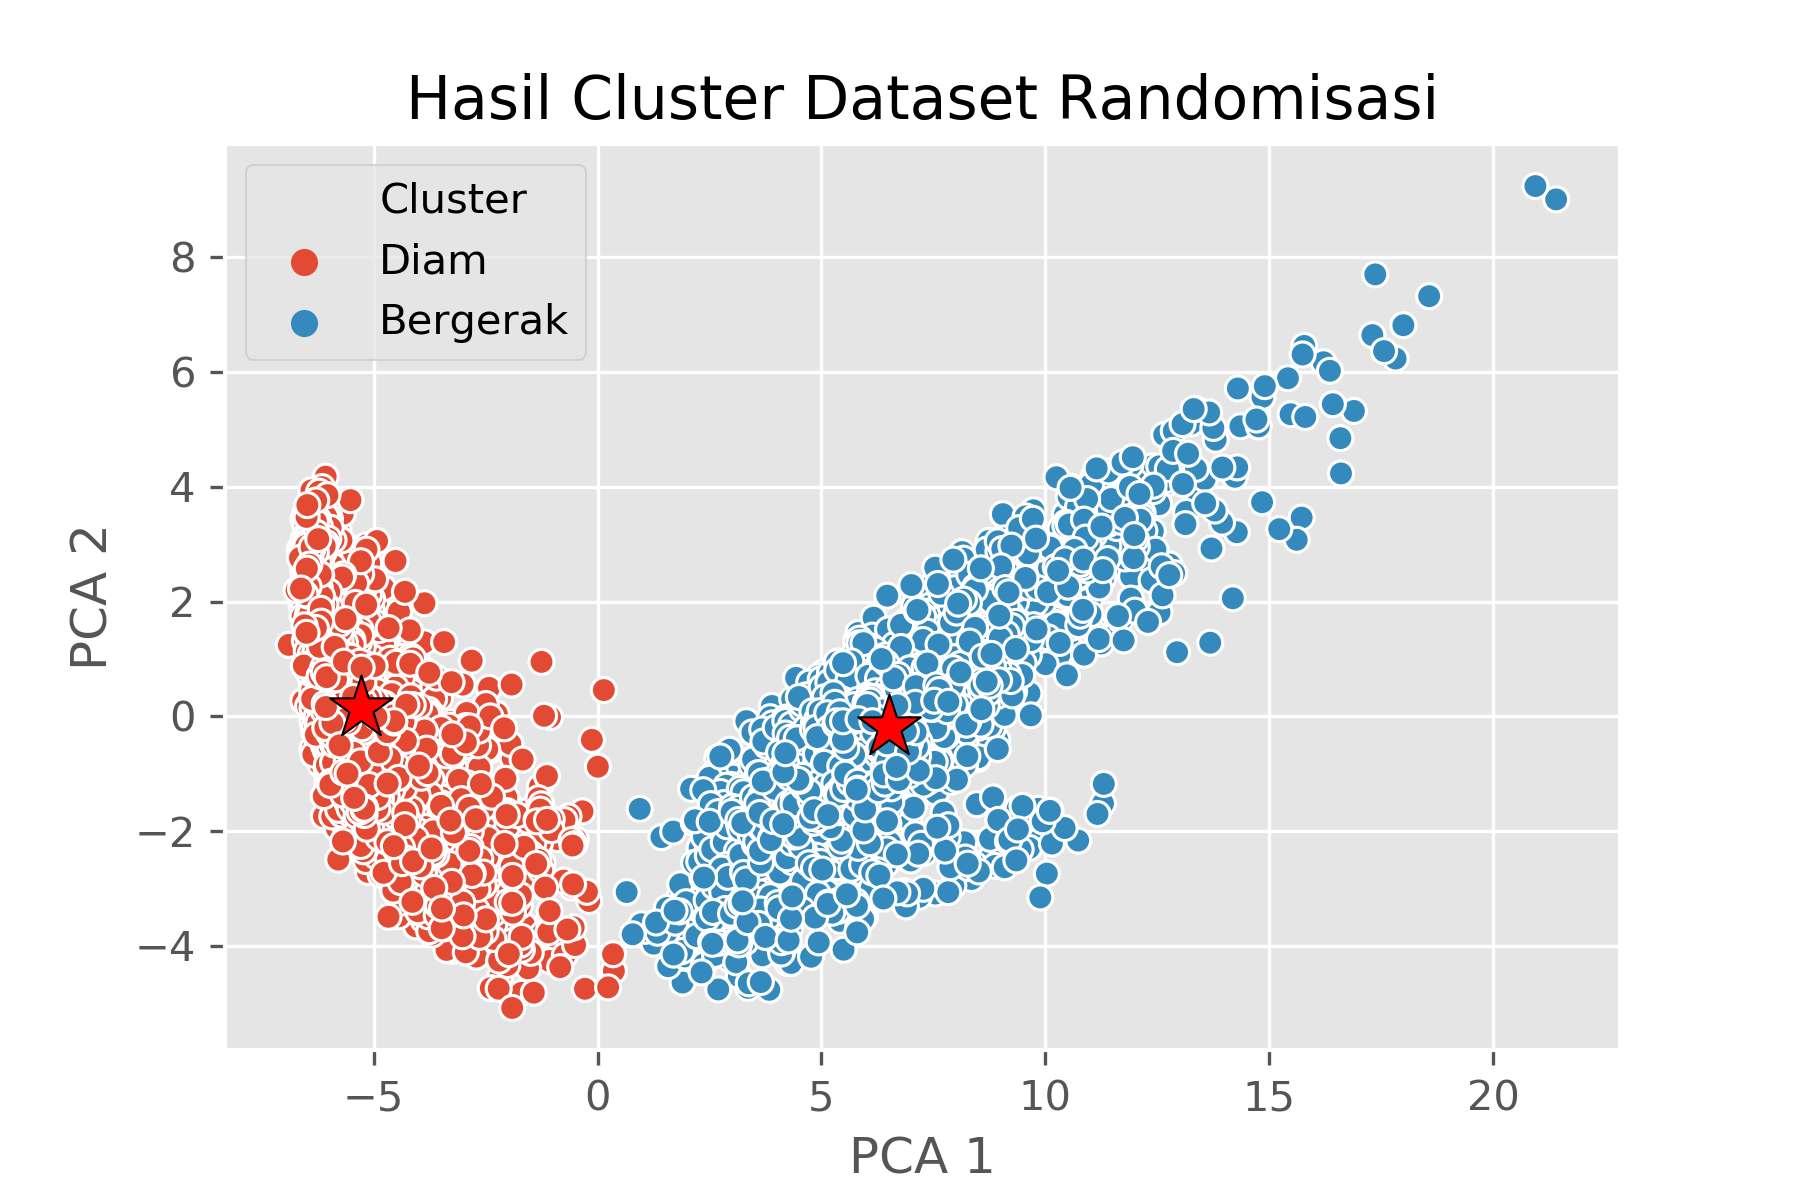
\includegraphics[scale=1]{kmeans_mobile_sensor_randomisasi}
	\caption{Visualisasi \textit{cluster} pada dataset yang telah diproyeksi}
	\label{fig:kmeans_mobile_sensor_randomisasi}
\end{figure}

Hasil \textit{clustering} menyatakan bahwa ada dua buah \textit{cluster} yaitu kelompok orang-orang yang diam dan kelompok orang-orang yang bergerak. Dapat dilihat pada kedua \textit{scatter plot} tersebut \textit{cluster} yang dihasilkan sama yaitu 2 \textit{cluster} walaupun ada sedikit perbedaan lokasi titik-titik yang ada pada kedua \textit{scatter plot} tersebut. \textit{Adjusted Rand Index} pada kedua model tersebut memiliki nilai sebesar 0.9994558701020273, mendekati angka 1. Dengan \textit{Adjusted Rand Index} sebesar itu dapat diartikan anggota \textit{cluster} pada setiap cluster antara kedua model tersebut hampir sama persis. Hal ini dikarenakan jarak Euclidean kedua buah dataset tidak rusak secara signifikan dan \textit{error}nya terkendali sesuai yang pengguna inginkan. Oleh karena itu, perangkat lunak berhasil menerapkan dengan baik teknik \textit{Random Projection Perturbation} untuk penambangan data \textit{clustering}.

\subsection{Pengujian Eksperimental}
\label{sec:pengujianeksperimental}